\section{Capitolo 6}



	\subsection{Esercizio 6.1}
	
Scrivere una function Matlab che generi la matrice sparsa $n \times n$ con $n > 10$, 
$
	A = 
	\begin{pmatrix}
		a_{11} & ... & a_{1n} \\
		. &  & . \\
		a_{n1} & ... & a_{nn}
	\end{pmatrix}
	\quad \text{con} 
$, con $a_{ij} =$ 
\begin{empheq}[left=\empheqlbrace]{align*}
	4,  & \text{se} & i = j \\
	-1, & \text{se} & i = j  \\
	-1, & \text{se} & i = j 
\end{empheq}
Utilizzare, a questo fine, la function Matlab \lstinline{spdiags}.
\PP
La function che genera la matrice $A$ è la seguente:
\lstinputlisting{./capitolo_6/sparse_diags.m}



	\subsection{Esercizio 6.2}
	
Utilizzare il metodo delle potenze per calcolarne l’autovalore dominante della matrice $A_n$ del precedente esercizio, con una approssimazione $tol = 10^{-5}$, partendo da un vettore con elementi costanti. Riempire, quindi, la seguente
tabella:
\begin{tabular}{|c|c|c|}
\hline
n & numero di iterazioni effettuate & stima autovalore\\
\hline
100 & & \\
200 & & \\
... & & \\
1000 & & \\
\hline
\end{tabular}
\PP
Il metodo delle potenze è implementato dalla seguente function:
\lstinputlisting{./capitolo_6/power_method.m}
la tabella viene generata usando lo script:
\lstinputlisting{./capitolo_6/exercise_6_2.m}
i risultati sono i seguenti:
\begin{tabular}{|c|c|r|}
	\hline
	n & iterazioni & stima $\lambda_1 $\\
	\hline
     	100  &  31  &  -5.9182  \\
     	200  &  49  &  -5.9760  \\
     	300  &  50  &  -5.9865  \\
     	400  &  44  &  -5.9905  \\
     	500  &  41  &  -5.9921  \\
     	600  &  40  &  -5.9928  \\
     	700  &  36  &  -5.9946  \\
     	800  &  37  &  -5.9944  \\
     	900  &  36  &  -5.9949  \\
    	1000  &  33  &  -5.9954  \\
    	\hline
\end{tabular}



	\subsection{Esercizio 6.3}

Utilizzare il metodo di Jacobi per risolvere il sistema lineare
\begin{equation*}
	A_n \mathbf{x} = \begin{pmatrix} 1 \\ \vdots \\ 1 \end{pmatrix}
\end{equation*}
dove $A_n$ è la matrice definita all'esercizio 6.1, con tolleranza $tol = 10^{-5}$, e partendo dal vettore nullo. Graficare il numero di iterazioni necessarie, rispetto alla dimensione $n$ del problema, con $n$ che varia da $100$ a $1000$ (con passo $20$).
\PP
La function che implementa il metodo di Jacobi è la seguente:
\lstinputlisting{./capitolo_6/jacobi.m}
lo script che la utilizza sugli $n = 100, 120, 140 ... 1000$ è:
\lstinputlisting{./capitolo_6/exercise_6_3.m}
che porta il seguente risultato, rappresentato in figura \ref{fig:6_3_jacobi}.\\
\begin{figure}[h!]
    \centering
    \includegraphics[scale=0.6]{./capitolo_6/exercise_6_3}
    \label{fig:6_3_jacobi}
    \caption{Numero di iterazioni del metodo di Jacobi necessarie per risolvere il sistema per n=100,120...1000}
\end{figure}



	\subsection{Esercizio 6.4}
	
Ripetere una procedura analoga a quella del precedente esercizio utilizzando il medodo di Gauss-Seidel.
\PP
La function che implementa il metodo di Gauss-Seidel è la seguente:
\lstinputlisting{./capitolo_6/gauss_seidel.m}
lo script che la utilizza sugli $n = 100, 120, 140 ... 1000$ è:
\lstinputlisting{./capitolo_6/exercise_6_4.m}
che porta il seguente risultato, rappresentato in figura \ref{fig:6_4_gauss}.\\
\begin{figure}[h!]
    \centering
    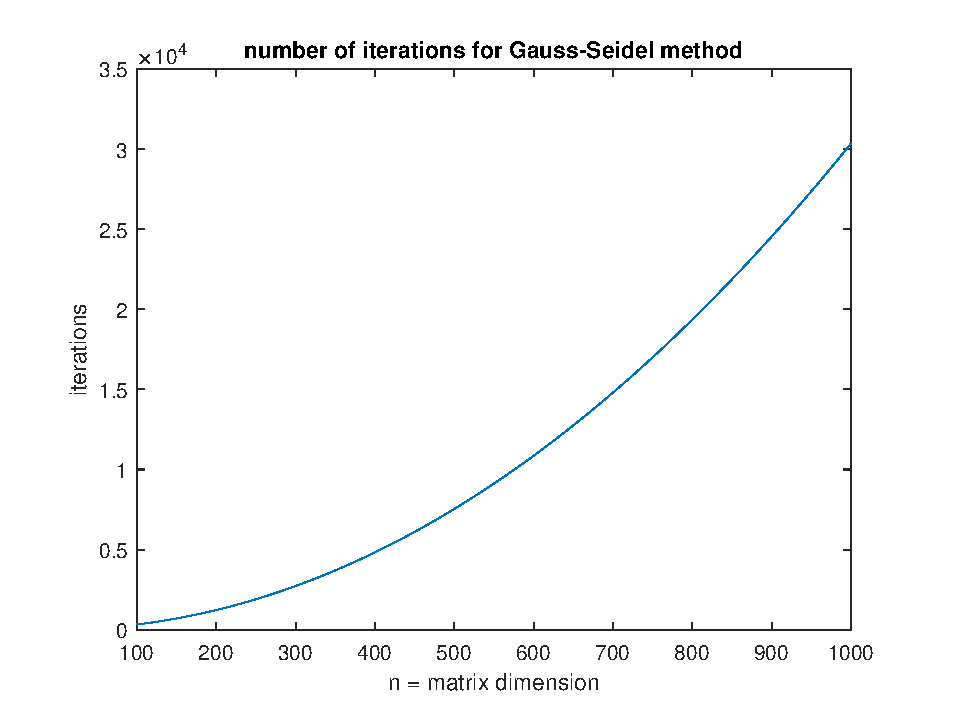
\includegraphics[scale=0.6]{./capitolo_6/exercise_6_4}
    \label{fig:6_4_gauss}
    \caption{Numero di iterazioni del metodo di Gauss-Seidel necessarie per risolvere il sistema per n=100,120...1000}
\end{figure}



	\subsection{Esercizio 6.5}
	
Con riferimento al sistema lineare
\begin{equation*}
	A_n \mathbf{x} = \begin{pmatrix} 1 \\ \vdots \\ 1 \end{pmatrix}
\end{equation*}
con $n = 1000$, graficare la norma dei residui, rispetto all’indice di iterazione, generati dai metodi di Jacobi e GaussSeidel.
Utilizzare il formato \lstinline{semilogy} per realizzare il grafico, corredandolo di opportune \textit{labels}.
\PP
Lo script che utilizza le functions di Jacobi e Gauss-Seidel e ne stampa su un grafico la norma dei residui ad ogni iterazione è il seguente:
\lstinputlisting{./capitolo_6/exercise_6_5.m}
Viene utilizzata una versione leggermente modificata dei due metodi, di cui cambia solo la firma ed il meccanismo interno (con cui ad ogni iterazione, oltre ai calcoli, si memorizza in un vettore $\norm{r}_i$):
\begin{lstlisting}[frame=single]
function [ nrs ] = nrs_gauss_seidel( A, b, tol )
%...

function [ nrs ] = nrs_jacobi( A, b, tol )
%...
\end{lstlisting}

La $\norm{r}$ per iterazione per i due metodi sono rappresentati nelle figure seguenti:
\begin{figure}[h!]
    \centering
    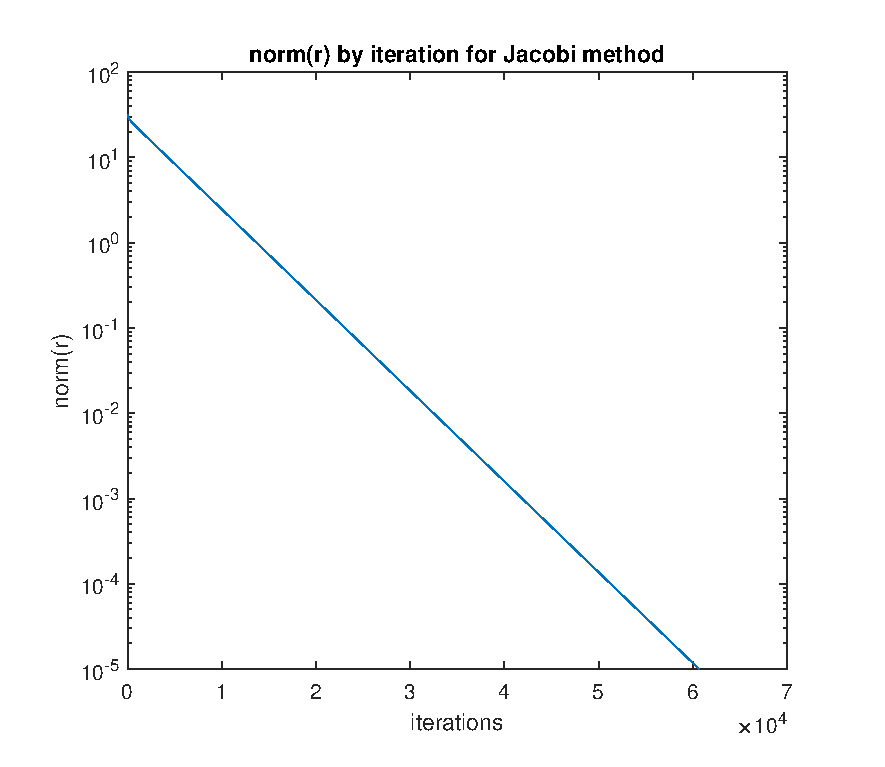
\includegraphics[scale=0.8]{./capitolo_6/exercise_6_5_jacobi}
    \label{fig:6_5_jacobi}
    \caption{$\norm{r}$ per iterazione del metodo di Jacobi}
\end{figure}
\begin{figure}[h!]
    \centering
    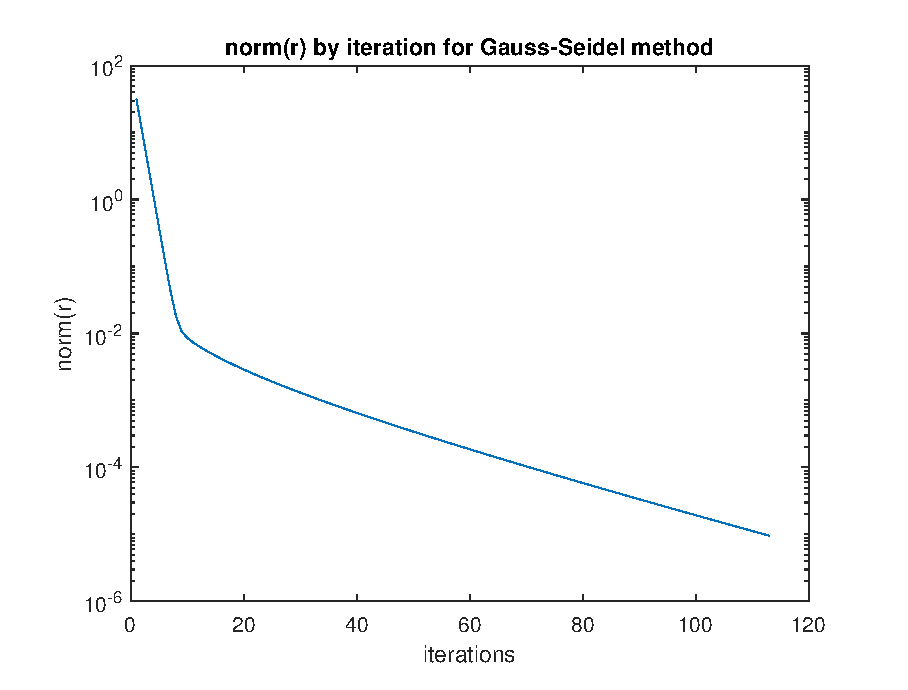
\includegraphics[scale=0.8]{./capitolo_6/exercise_6_5_gauss}
    \label{fig:6_5_gauss}
    \caption{$\norm{r}$ per iterazione del metodo di Gauss-Seidel}
\end{figure}